\begin{definition}
    Vertices represent random variables and edges represent dependencies between variables.
\end{definition}

\subsection{Junction}
\begin{definition}
    A \textbf{junction} $\mathcal{J}$ consists of three vertices, $X_1$, $X_2$, and $X_3$, connected by two edges, $e_1$ and $e_2$:
    \customFigure[0.5]{../Images/L6_2.png}{}
    \begin{itemize}
        \item $X_1$ and $X_2$ are not independent, $X_2$ and $X_3$ are not independent, but when is $X_1$ and $X_3$ independent?
    \end{itemize}
\end{definition}

\subsubsection{Causal Chain}
\begin{definition}
    A causal chain is a junction $\mathcal{J}$ s.t. 
    \customFigure[0.5]{../Images/L6_3.png}{}
    \begin{itemize}
        \item $X_1$ and $X_3$ are not independent (unconditionally), but are independent given $X_2$.
    \end{itemize}
\end{definition}

\begin{notes}
    \begin{itemize}
        \item \textbf{Analogy:}  Given $X_2$, $X_1$ and $X_3$ are independent. Why? $X_2$'s door closes when you know $X_2$, so $X_1$ and $X_3$ are independent.
        \item \textbf{Distinction b/w Causal and Dependence:} $X_1$ and $X_2$ are dependent. However, from a causal perspective, $X_1$ is influencing $X_2$ (i.e. $X_1 \rightarrow X_2$).
    \end{itemize}
\end{notes}

\subsubsection{Common Cause}
\begin{definition}
    A common cause is a junction $\mathcal{J}$ s.t.
    \customFigure[0.5]{../Images/L6_4.png}{}
    \begin{itemize}
        \item $X_1$ and $X_3$ are not independent (unconditionally), but are independent given $X_2$.
    \end{itemize}
\end{definition}

\begin{notes}
    \begin{itemize}
        \item \textbf{Analogy:} Given $X_2$, $X_1$ and $X_3$ are independent. Why? Consider the following example:
        \begin{itemize}
            \item Let $X_2$ represent whether a person smokes or not, $X_1$ represent whether they have yellow teeth, $X_3$ represent whether they have lung cancer.
        \end{itemize}
        \item Without knowing $X_2$, observing $X_1$ provides information about $X_3$ because yellow teeth are associated with smoking, which in turn increases the likelihood of lung cancer. 
        \item If $X_2$ is known, then knowing whether a person has yellow teeth provides no additional information about whether they have lung cancer beyond what is already known from smoking status. 
    \end{itemize}
\end{notes}


\subsubsection{Common Effect}
\begin{definition}
    A common effect is a junction $\mathcal{J}$ s.t.
    \customFigure[0.5]{../Images/L6_5.png}{}
    \begin{itemize}
        \item $X_1$ and $X_3$ are independent (unconditionally), but are not independent given $X_2$ or any of $X_2$'s descendents.
    \end{itemize}
\end{definition}

\begin{notes}
    \begin{itemize}
        \item \textbf{Analogy:} Consider the following example:
        \begin{itemize}
            \item Let $X_2$ represent whether the grass is wet, $X_1$ represent whether it rained, $X_3$ represent whether the sprinkler was on.
        \end{itemize}
        \item Without knowing whether the grass is wet ($X_2$), the occurrence of rain ($X_1$) and the sprinkler being on ($X_3$) are independent events. The rain may occur regardless of the sprinkler, and vice versa.
        \item However, once we observe that the grass is wet ($X_2$), the two events become dependent:
        \begin{itemize}
            \item If we learn that the sprinkler was not on, then the wet grass must have been caused by rain.
            \item If we learn that it did not rain, then the wet grass must have been caused by the sprinkler.
        \end{itemize}
    \end{itemize}
\end{notes}
\newpage

\section{Dependence Separation}
\subsection{Independence}
\begin{theorem}
    Any two variables, $X_1$ and $X_2$, in a Bayesian network, $\mathcal{B} = (\mathcal{V}, \mathcal{E})$, are independent given $\mathcal{K} \subseteq \mathcal{V}$ if every undirected path is blocked.
\end{theorem}

\subsubsection{Blocked Undirected Path}
\begin{definition}
    An undirected path,
    \[
    p = \langle (X_1, e_1, X_2), \dots, (X_{|p|-1}, e_{|p|-1,|p|}, X_{|p|}) \rangle,
    \]
    \customFigure[0.5]{../Images/L6_13.png}{}
    is \textbf{blocked} given $\mathcal{K} \subseteq \mathcal{V}$ if any of its junctions,

    \[
    \mathcal{J}^{(n)} = \{(X_{n-1}, X_n, X_{n+1}), (e_{n-1}, e_n)\},
    \]
    is blocked given $\mathcal{K}$.
\end{definition}

\subsubsection{Blocked Junction}
\begin{definition}
    $\mathcal{J} = (\{X_1, X_2, X_3\}, \{e_1, e_2\})$ is \textbf{blocked} given $\mathcal{K} \subseteq \mathcal{V}$ if $X_1$ and $X_3$ are independent given $\mathcal{K}$.
\end{definition}

\subsection{Consequence of Dependence Separation}
\begin{theorem}
    For any variable, $X \in \mathcal{V}$, it can be shown that $X$ is independent of $X$'s non-descendants, $\mathcal{V} \setminus \operatorname{des}(X)$, given $X$'s parents, $\operatorname{pts}(X)$.
\end{theorem}

\begin{notes}
    \customFigure[0.5]{../Images/L6_8.png}{}
    \begin{itemize}
        \item Given $X$'s parent, apply junction rules to determine that $X$ is independent of its non-descendants.
        \item $\mathcal{J} = \{(Z_1, \text{pt}(X), X), (e_1,e)\}$ shows that $Z_1$ and $X$ are independent given $\text{pt}(X)$ (causal chain).
        \item $\mathcal{J} = \{(Z_2, \text{pt}(X), X), (e_2,e)\}$ shows that $Z_2$ and $X$ are independent given $\text{pt}(X)$ (common cause).
        \item Given $\text{ch}(X)$'s parent, apply junction rules to determine that $\text{ch}(X)$ is independent of its non-descendants.
        \item $\mathcal{J} = \{\text{pt}(X),X, \text{ch}(X)), (e,e')\}$ shows that $\text{pt}(X)$ and $\text{ch}(X)$ are independent given $X$ (causal chain).
        \item Given $Z_4$'s parent, apply junction rules to determine that $Z_4$ is independent of its non-descendants.
        \item $\mathcal{J} = \{X, \text{ch}(X), Z_4, (e',e_4)\}$ shows that $X$ and $Z_4$ are independent given $\text{ch}(X)$ (causal chain).
    \end{itemize}
\end{notes}

\subsection{Flow Chart}
\begin{summary}
    \begin{center}
        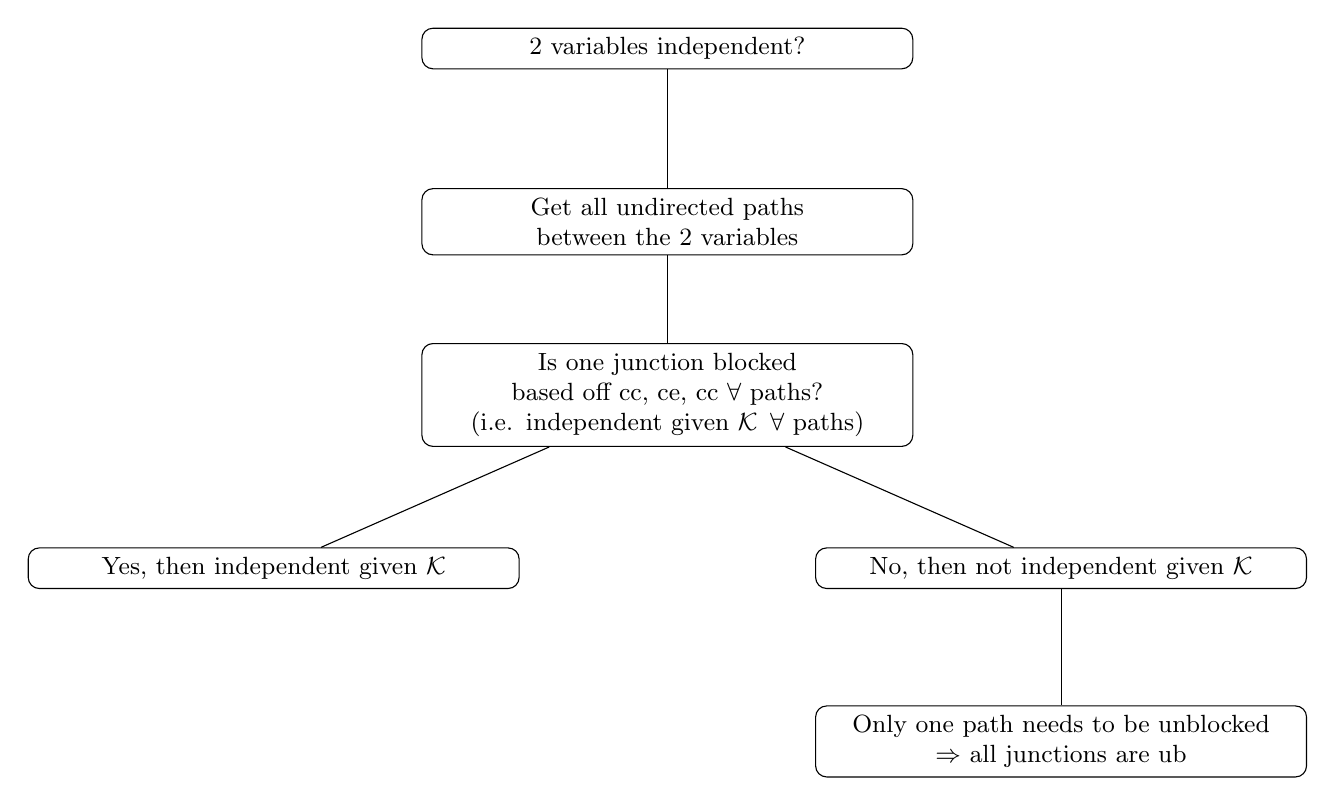
\begin{tikzpicture}[
            every node/.style={
                rectangle, draw, align=center, text width=6cm, rounded corners, font=\small
            },
            level distance=2.2cm,
            sibling distance=10cm
        ]
        
        \node {2 variables independent?}
          child {node {Get all undirected paths between the 2 variables}
            child {node {Is one junction blocked based off cc, ce, cc $\forall$ paths?\\
                        (i.e. independent given $\mathcal{K} \; \forall$ paths)}
              child {node {Yes, then independent given $\mathcal{K}$}}
              child {node {No, then not independent given $\mathcal{K}$}
                child {node {Only one path needs to be unblocked \\
                $\Rightarrow$ all junctions are ub}}
              }
            }
          };
        
    \end{tikzpicture}
    \end{center}
\end{summary}
\newpage

\subsection{Canonical Problems}
\subsubsection{Undirected Path Blocked?}
\begin{process}
    \begin{enumerate}
        \item \textbf{Given:} Undirected path $p$ and $\mathcal{K}$
        \item Check if any of the junctions on the undirected path are blocked given $\mathcal{K}$.
        \begin{itemize}
            \item i.e. Check if $X_1$ and $X_3$ of the junction are independent given $\mathcal{K}$.
        \end{itemize}
    \end{enumerate}
\end{process}

\subsubsection{Independence}
\begin{process}
    \begin{enumerate}
        \item Given a Bayesian network w/ 2 variables to find independence.
        \item Find all undirected paths between the 2 variables in the Bayesian network.
        \item Identify a set of variables, $\mathcal{K}$, that block at least one junction in all undirected paths.
        \begin{itemize}
            \item Test a junction by seeing junction given relationships. 
        \end{itemize}
        \item If all undirected paths are blocked, then the 2 variables are independent given $\mathcal{K}$.
    \end{enumerate}
\end{process}

\begin{warning}
    \begin{itemize}
        \item \textbf{Common effect:} Blocked by default. 
        \begin{itemize}
            \item \textbf{Decesdents: of a common effect:} Outward arrows from a common effect node as given it may not be blocked.
            \item \textbf{Subset:} If $\mathcal{K}$ includes variables that cause all undirected paths to be blocked, then variables are independent. BUT be careful of common effect, in which it is blocked by default so YOU DONT INCLUDE IT IN $\mathcal{K}$.
        \end{itemize}
        \item Cyclic paths are not blocked by default.
    \end{itemize}
\end{warning}

\subsubsection{Find all Subsets}
\begin{notes}
    \begin{itemize}
        \item For each full independence set, add an OR b/w each subset. Be careful of common effect. 
    \end{itemize}
\end{notes}
\newpage 

\begin{example}
    \begin{enumerate}
        \item \textbf{Given:} Bayesian network.
        \customFigure[0.25]{../Images/L6_7.png}{}
        \item \textbf{Problem:} $A$ and $E$ are 
        \begin{itemize}
            \item independent if $\mathcal{K}=$
            \item not necessarily independent for $\mathcal{K}=$
        \end{itemize}
        \item \textbf{Soln:}
        \begin{enumerate}
            \item \textbf{Undirected Paths:}
            \begin{itemize}
                \item $A \to G \to H \to B \to E$
                \item $A \to G \to D \to B \to E$
                \item $A \to C \to F \to B \to E$
                \item $A \to C \to D \to B \to E$
            \end{itemize}
        \end{enumerate}
    \end{enumerate}
\end{example}
\newpage

\begin{example}
    \textbf{Independent:}
    \begin{center}
        \begin{tabular}{c}
            \toprule
            $\mathcal{K}$ \\
            \midrule
            $\{G,C\}$ \\
            \multicolumn{1}{p{\linewidth}}{
                \begin{itemize}
                    \item $A \iff G \iff H \iff B \iff E$ is blocked given $\mathcal{K}$ since $\mathcal{J} = \{(A,G,H),(e_1,e_2)\}$ is blocked given $G$ since $A,H$ independent given $G$ (causal chain)
                    \item $A \iff G \iff D \iff B \iff E$ is blocked given $\mathcal{K}$ since $\mathcal{J} = \{(A,G,D),(e_1,e_2)\}$ is blocked given $G$ since $A,D$ independent given $G$ (causal chain)
                    \item $A \iff C \iff F \iff B \iff E$ is blocked given $\mathcal{K}$ since $\mathcal{J} = \{(A,C,F),(e_1,e_2)\}$ is blocked given $C$ since $A,F$ independent given $C$ (causal chain) 
                    \item $A \iff C \iff D \iff B \iff E$ is blocked given $\mathcal{K}$ since $\mathcal{J} = \{(A,C,D),(e_1,e_2)\}$ is blocked given $C$ since $A,D$ independent given $C$ (causal chain) 
                \end{itemize}} \\
            \midrule
            $\{D,F\}$ \\
            \multicolumn{1}{p{\linewidth}}{
                \begin{itemize}
                    \item $A \iff G \iff H \iff B \iff E$ is blocked given $\mathcal{K}$ since $\mathcal{J} = \{(G,H,B),(e_1,e_2)\}$ is blocked NOT given $H$ since $G,B$ independent NOT given $H$ (common effect)
                    \item $A \iff G \iff D \iff B \iff E$ is blocked given $\mathcal{K}$ since $\mathcal{J} = \{(G,D,B),(e_1,e_2)\}$ is blocked given $D$ since $G,B$ independent given $D$ (causal chain)
                    \item $A \iff C \iff F \iff B \iff E$ is blocked given $\mathcal{K}$ since $\mathcal{J} = \{(C,F,B),(e_1,e_2)\}$ is blocked given $F$ since $C,B$ independent given $F$ (causal chain)
                    \item $A \iff C \iff D \iff B \iff E$ is blocked given $\mathcal{K}$ since $\mathcal{J} = \{(C,D,B),(e_1,e_2)\}$ is blocked given $D$ since $C,B$ independent given $D$ (causal chain)
                \end{itemize}} \\
            \toprule
        \end{tabular}
    \end{center}
    \vspace{1em}

    \textbf{Not Necessarily Independent:}
    \begin{center}
        \begin{tabular}{c}
            \toprule
            $\mathcal{K}$ \\
            \midrule
            $\{H,D,F\}$ \\
            \multicolumn{1}{p{\linewidth}}{
                \begin{itemize}
                    \item $A \iff G \iff H \iff B \iff E$ is unblocked given $\mathcal{K}$ since $\mathcal{J} = \{(G,H,B),(e_1,e_2)\}$ is unblocked given $H$ since $G,B$ not independent given $H$ (common effect)
                    \item $A \iff G \iff D \iff B \iff E$ is blocked given $\mathcal{K}$ since $\mathcal{J} = \{(G,D,B),(e_1,e_2)\}$ is blocked given $D$ (causal chain) since $G,B$ independent given $D$ (causal chain)
                    \item $A \iff C \iff F \iff B \iff E$ is blocked given $\mathcal{K}$ since $\mathcal{J} = \{(C,F,B),(e_1,e_2)\}$ is blocked given $F$ since $C,B$ independent given $F$ (causal chain)
                    \item $A \iff C \iff D \iff B \iff E$  is blocked given $\mathcal{K}$ since $\mathcal{J} = \{(C,D,B),(e_1,e_2)\}$ is blocked given $D$ since $C,B$ independent given $D$ (causal chain)
                \end{itemize}} \\
            \midrule
            \toprule
        \end{tabular}
    \end{center}
\end{example}
\newpage

\begin{example}
    Determine all subsets of $\{B,C,D,F,G,H\}$ for which $A$ and $E$ are independent. 
    \customFigure[0.25]{../Images/LR_1.png}{}
    \begin{enumerate}
        \item \textbf{Undirected Paths:}
        \begin{itemize}
            \item $A \to G \to H \to B \to E$
            \item $A \to G \to D \to B \to E$
            \item $A \to C \to F \to B \to E$
            \item $A \to C \to D \to B \to E$
        \end{itemize}
    \end{enumerate}
    \begin{center}
        \begin{tabular}{c}
            \toprule
            $\mathcal{K}$ \\
            \midrule
            $\{B\}$ (Any subset that contains $B$ will be independent) \\
            \multicolumn{1}{p{\linewidth}}{
                \begin{itemize}
                    \item $AGHBE$ is b given $\mathcal{K}$ since $\mathcal{J} = \{(H,B,E),(e_1,e_2)\}$ is b since $H,E$ indep. given $B$ (causal chain)
                    \item $AGDBE$ is b given $\mathcal{K}$ since $\mathcal{J} = \{(D,B,E),(e_1,e_2)\}$ is b since $D,E$ indep. given $B$ (causal chain)
                    \item $ACFBE$ is b given $\mathcal{K}$ since $\mathcal{J} = \{(F,B,E),(e_1,e_2)\}$ is b since $F,E$ indep. given $B$ (causal chain) 
                    \item $ACDBE$ is b given $\mathcal{K}$ since $\mathcal{J} = \{(D,B,E),(e_1,e_2)\}$ is b since $D,E$ indep. given $B$ (causal chain) 
                \end{itemize}} \\
            \midrule
            $\{C\}$ (Not independent) \\
            \multicolumn{1}{p{\linewidth}}{
                \begin{itemize}
                    \item $AGDBE$ is ub given $\mathcal{K}$ since $\mathcal{J} = \{(D,B,E),(e_1,e_2)\}$ is ub since $D,E$ NOT indep. given $\mathcal{K}$ (causal chain)
                \end{itemize}} \\
            \midrule
            $\{D\}$ (Not indepedent) \\
            \multicolumn{1}{p{\linewidth}}{
                \begin{itemize}
                    \item $ACFBE$ is ub given $\mathcal{K}$ since $\mathcal{J} = \{(F,B,E),(e_1,e_2)\}$ is ub since $F,E$ NOT indep. given $\mathcal{K}$ (causal chain)
                \end{itemize}} \\
            \midrule
            $\{F\}$ (Not independent) \\
            \multicolumn{1}{p{\linewidth}}{
                \begin{itemize}
                    \item $AGDBE$ is ub given $\mathcal{K}$ since $\mathcal{J} = \{(D,B,E),(e_1,e_2)\}$ is ub since $D,E$ NOT indep. given $\mathcal{K}$ (causal chain)
                \end{itemize}} \\
            \midrule
            $\{G\}$ (Not independent) \\
            \multicolumn{1}{p{\linewidth}}{
                \begin{itemize}
                    \item $ACFBE$ is ub given $\mathcal{K}$ since $\mathcal{J} = \{(F,B,E),(e_1,e_2)\}$ is ub since $F,E$ NOT indep. given $\mathcal{K}$ (causal chain)
                \end{itemize}} \\
            \midrule
            $\{H\}$ (Not independent) \\
            \multicolumn{1}{p{\linewidth}}{
                \begin{itemize}
                    \item $ACFBE$ is ub given $\mathcal{K}$ since $\mathcal{J} = \{(F,B,E),(e_1,e_2)\}$ is ub since $F,E$ NOT indep. given $\mathcal{K}$ (common effect)
                \end{itemize}} \\
            \toprule
        \end{tabular}
    \end{center}
\end{example}
\newpage

\begin{example}
    \begin{center}
        \begin{tabular}{c}
            \toprule
            $\mathcal{K}$ \\
            \midrule
            $\{C,D\}$ (Any subset that contains $C$ and $D$ except $H$ will be independent) \\
            \multicolumn{1}{p{\linewidth}}{
                \begin{itemize}
                    \item $AGHBE$ is b given $\mathcal{K}$ since $\mathcal{J} = \{(G,H,B),(e_1,e_2)\}$ is b since $G,B$ indep. not given $H$ (common effect)
                    \item $AGDBE$ is b given $\mathcal{K}$ since $\mathcal{J} = \{(G,D,B),(e_1,e_2)\}$ is b since $G,B$ indep. given $D$ (causal chain)
                    \item $ACFBE$ is b given $\mathcal{K}$ since $\mathcal{J} = \{(A,C,F),(e_1,e_2)\}$ is b since $A,F$ indep. given $C$ (causal chain)
                    \item $ACDBE$ is b given $\mathcal{K}$ since $\mathcal{J} = \{(A,C,D),(e_1,e_2)\}$ is b since $A,D$ indep. given $C$ (causal chain)
                \end{itemize}} \\
            \midrule
            $\ldots$ \\
            \toprule
        \end{tabular}
    \end{center}
\end{example}
\newpage

\begin{example}
    \begin{enumerate}
        \item \textbf{Given:}
        \customFigure[0.25]{../Images/FE23_7.png}{}
        \item \textbf{Problem 1:} Is it gauranteed that $A \perp C$?
        \item \textbf{Solution 1:} True b/c all undirected paths are blocked.
        \begin{enumerate}
            \item ADEFC is b since $\mathcal{J} = \{(D,E,F),(e_1,e_2)\}$ is b since $D$, $F$ indep. NOT given $E$ (common effect)
            \item ADGHEFC is b since $\mathcal{J} = \{(G,H,E),(e_1,e_2)\}$ is b since $G,E$ indep. NOT given $H$ (common effect)
            \item ADGHIEFC is b since $\mathcal{J} = \{(H,I,E),(e_1,e_2)\}$ is b since $H,E$ indep. NOT given $I$ (common effect)
        \end{enumerate}
        \vspace{1em}
        \item \textbf{Problem 2:} Is it gauranteed that $B \perp C \mid I$?
        \item \textbf{Solution 2:} False b/c BEFC is ub. 
        \begin{enumerate}
            \item BEFC is ub since $\mathcal{J} = \{(B,E,F),(e_1,e_2)\}$ is ub since $B,F$ NOT indep. given $E$'s descendent, $I$ (common effect)
        \end{enumerate}
        \vspace{1em}
        \item \textbf{Problem 3:} Is it gauranteed that $D \perp I \mid \{E,G\}$?
        \item \textbf{Solution 3:} True b/c all undirected paths are blocked.
        \begin{enumerate}
            \item DEI is b since $\mathcal{J} = \{(D,E,I),(e_1,e_2)\}$ is b since $D,I$ indep. given $E$ (causal chain)
            \item DEHI is b since $\mathcal{J} = \{(D,E,H),(e_1,e_2)\}$ is b since $D,H$ indep. given $E$ (causal chain)
            \item DGHI is b since $\mathcal{J} = \{(D,G,H),(e_1,e_2)\}$ is b since $D,H$ indep. given $G$ (causal chain)
            \item DGHEI is b since $\mathcal{J} = \{(D,G,H),(e_1,e_2)\}$ is b since $D,H$ indep. given $G$ (causal chain)
        \end{enumerate}
        \vspace{1em}
        \item \textbf{Problem 4:} Is it gauranteed that $C \perp H \mid G$?
        \item \textbf{Solution 4:} False b/c CFEH is ub.
        \begin{enumerate}
            \item CFEH is ub since $\mathcal{J} = \{(C,F,E),(e_1,e_2)\}$ is ub since $C,E$ NOT indep. given $G$ (causal chain)
        \end{enumerate}
    \end{enumerate}
\end{example}

\begin{example}
    \begin{enumerate}
        \item \textbf{Problem 5:} Suppose each variable is binary. What is the size of the domain of the joint distribution b/w the variables?
        \item \textbf{Solution 5:}
        \begin{enumerate}
            \item Since 9 variables, each with 2 values, the size of the domain of the joint distribution is $2^9 = 512$.
        \end{enumerate}
        \vspace{1em}
        \item \textbf{Problem 6:} Suppose each variable is binary. What is the min \# of values that actually need to be stored to represent the joint distribution entirely based on the Bayesian network? Use the fact that probability distributions are normalized.
        \item \textbf{Solution 6:} 1+1+1+2+8+2+2+4+4 = 25 values need to be stored.
        \begin{enumerate}
            \item $P(A)$, $P(B)$, $P(C)$ has 1 value each 
            \begin{itemize}
                \item Since $P(\#)$ can represent 2 values, i.e. $P(0) = 1-P(1)$, so only need to store 1 value.
            \end{itemize}
            \item $P(D \mid A)$, $P(F \mid C)$, $P(G \mid D)$ has 2 values each
            \begin{itemize}
                \item Same idea, can take the complement of the other value for 4 values.
            \end{itemize}
            \item $P(H \mid G,E)$, $P(I \mid E,H)$ has 4 values each
            \begin{itemize}
                \item Same idea, can take the complement of the other value for 8 values.
            \end{itemize}
            \item $P(E \mid D,B,F)$ has 8 values 
            \begin{itemize}
                \item Same idea, can take the complement of the other value for 16 values.
            \end{itemize}
        \end{enumerate}
    \end{enumerate}
\end{example}

